\chapter{系统的频率分析}

上一章介绍了傅里叶变换,也介绍了信号的傅里叶变换和信号的频域分析。

本章用傅里叶变换分析系统。
首先分析频域角度上的系统响应,即“系统的频率响应”,给出“频率响应函数”概念。
再以RC电路为例,在频域角度分析系统特性。
最后用频率响应函数定义理想滤波器。

本章要点:
\begin{itemize}
    \item 系统的频率响应。
    \item 频率响应函数。
    \item 理想滤波器。
    \item Nuquist采样定理
\end{itemize}

\newpage
\section{系统的频率响应}

本节在频域角度,讨论系统如何对输入作用产生输出,介绍系统的频域响应定理与频率响应函数,并给出快速求解系统频率响应函数的方法。

本节要点:
\begin{itemize}
    \item 掌握系统频率响应的概念;
    \item 理解频率响应函数的概念和意义;
    \item 掌握频率响应函数的求解方法。
\end{itemize}

%============================================================
\subsection{频域响应定理与频率响应函数}

\begin{theorem}[系统的频域响应定理]
若一个零状态LTI系统满足绝对稳定的条件,即$\int_{-\infty}^{+\infty}{\left| h\left( t \right) \right|dt}$收敛,则系统对于任意非周期信号$x\left( t \right) $在时域的输出可以表示为卷积:
\[
y\left( t \right) =x\left( t \right) \ast h\left( t \right)
\]
在频域的输出可以表示为傅里叶变换的乘积:
\[
Y\left( \omega \right) =X\left( \omega \right) \cdot H\left( \omega \right)
\]
\begin{itemize}
    \item $x\left( t \right) ,y\left( t \right) $:输入输出信号的时域表达式;
    \item $h\left( t \right) $:系统的冲激响应;
    \item $X\left( \omega \right) ,Y\left( \omega \right) $:输入输出信号的傅里叶变换;
    \item $H\left( \omega \right) $:{\bf 系统的频率响应函数}(frequency response function),或称{\bf 系统函数}(system function),即$h\left( t \right) $的傅里叶变换。
\end{itemize}
\end{theorem}

这表明,一个绝对稳定的LTI系统对任何输入的信号,系统会单独作用其各个频率分量的幅度和相位:
\begin{align*}
&\left| Y\left( \omega \right) \right|=\left| X\left( \omega \right) \right|\cdot \left| H\left( \omega \right) \right| \\
&\angle Y\left( \omega \right) =\angle X\left( \omega \right) +\angle H\left( \omega \right)
\end{align*}
以简单的正弦信号为例,若信号$x\left( t \right) =A\cos \left( \omega _0t+\varphi \right) $,则输出:
\[
y\left( t \right) =A\left| H\left( \omega _0 \right) \right|\cos \left( \omega _0t+\varphi +\angle H\left( \omega _0 \right) \right)
\]
\begin{itemize}
    \item 若系统是无源系统,则$\left| H\left( \omega _0 \right) \right|\leqslant 1$,表示衰减,若系统为有源系统,对应$\left| H\left( \omega _0 \right) \right|>1$,表示放大;
    \item 由于因果性,系统都会将相位往后拉$\angle H\left( \omega _0 \right) $。
\end{itemize}

从定义上来说,$H\left( \omega \right) $是系统的$h\left( t \right) $的傅里叶变换,$h\left( t \right) $是系统对$\delta \left( t \right) $的响应。
由于$\delta \left( t \right) \leftrightarrow 1$,所以从频域上看,$H\left( \omega \right) $是系统对于输入$X\left( \omega \right) =1$的响应。
明白了这一点,也就明白了为什么$H\left( \omega \right) $会被称为“频率响应函数”,指的是系统对各个频率的响应。

%============================================================
\subsection{时域响应和频域响应}

至此,时域响应和频域响应讨论完毕。

在时域我们通过卷积模型描述系统,系统的输出为冲激响应对输入进行卷积运算的结果,不同的系统表现为不同的$h\left( t \right) $。
在频域我们通过傅里叶变换描述系统,输出为频率响应和输入信号的乘积,不同的系统表现为不同的$H\left( \omega \right) $。
无论是卷积模型还是傅里叶变换,本质上都是系统微分方程的反映,是微分方程的冲激函数的解在时域和频域的不同体现。
\[
y\left( t \right) \overset{h\left( t \right) \leftrightarrow H\left( \omega \right)}{=}\begin{cases}
	x\left( t \right) \ast h\left( t \right)\\
	\mathscr{F} ^{-1}\left[ H\left( \omega \right) \cdot X\left( \omega \right) \right]\\
\end{cases}
\]

%============================================================
\subsection{频率响应函数的求解}

\begin{tcolorbox}
系统的频率响应函数可以从定义上求解,但这涉及求解微分方程,特别是高阶的微分方程,几乎无解。
这里给出一个求解的方法。
\end{tcolorbox}

若有限维度LTI系统的微分方程如下:
\[
y^{\left( n \right)}\left( t \right) +\sum_{k=0}^{n-1}{A_ky^{\left( k \right)}\left( t \right)}=\sum_{k=0}^m{B_kx^{\left( k \right)}\left( t \right)}
\]
根据傅里叶变换的导数性质$\frac{d^nx\left( t \right)}{dt^n}\leftrightarrow \left( i\omega \right) ^n\cdot X\left( \omega \right) $,两边取傅里叶变换:
\[
\left( i\omega \right) ^nY\left( \omega \right) +\sum_{k=0}^{n-1}{A_k\left( i\omega \right) ^kY\left( \omega \right)}=\sum_{k=0}^m{B_k\left( i\omega \right) ^kX\left( \omega \right)}
\]
整理后得到:
\[
H\left( \omega \right) =\frac{\sum_{k=0}^m{B_k\left( i\omega \right) ^k}}{\left( i\omega \right) ^n+\sum_{k=0}^{n-1}{A_k\left( i\omega \right) ^k}}
\]

\begin{tcolorbox}
由于$i$代表虚数符号,所以进入到傅里叶章节后用$k$作为连加的序数。
\end{tcolorbox}

%============================================================
\subsection{例}

\begin{example}
如下RC电路,设电压源为输入,电容两端电压为输出,分析系统的频率响应函数。
\begin{figure}[h]
\centering
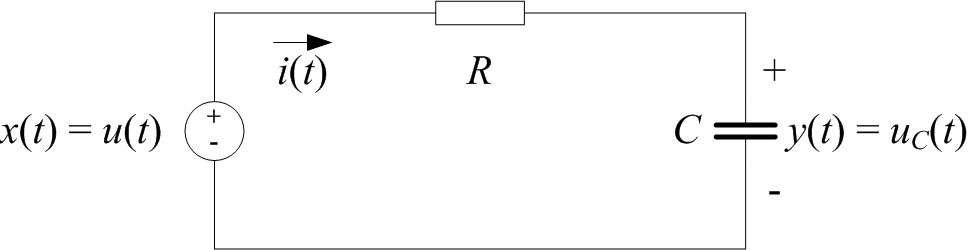
\includegraphics[height=2cm]{1.5.1-1.png}
\end{figure}
\end{example}

根据之前对该电路的分析,系统微分方程有:
\[
\frac{dy}{dt}+\frac{1}{RC}y=\frac{1}{RC}x
\]
直接运用上面的推导结论,有:
\[
H\left( \omega \right) =\frac{\sum_{k=0}^m{B_k\left( i\omega \right) ^k}}{\left( i\omega \right) ^n+\sum_{k=0}^{n-1}{A_k\left( i\omega \right) ^k}}=\frac{\frac{1}{RC}\left( i\omega \right) ^0}{\left( i\omega \right) ^1+\frac{1}{RC}\left( i\omega \right) ^0}=\frac{\frac{1}{RC}}{i\omega +\frac{1}{RC}}
\]
用最原始的方法,求解微分方程->求解冲激响应->获得频率响应函数。
求解微分方程及冲激响应:
\begin{align*}
&y=\frac{1}{RC}e^{-\frac{t}{RC}}\int_0^t{e^{\frac{\tau}{RC}}x\left( \tau \right) d\tau} \\
&h=\left. y \right|_{x=\delta}=\frac{1}{RC}e^{-\frac{t}{RC}}\int_0^t{e^{\frac{\tau}{RC}}\delta \left( \tau \right) d\tau}=\frac{1}{RC}e^{-\frac{t}{RC}}
\end{align*}
求解频率响应函数:
\begin{align*}
&\because e^{-bt}u\left( t \right) \leftrightarrow \frac{1}{b+i\omega} \\
&\therefore H\left( \omega \right) =\frac{1}{RC}\frac{1}{\frac{1}{RC}+i\omega}
\end{align*}

~

\begin{example}
设有弹簧减震装置,系统的微分方程为$x-D\frac{dy}{dt}-Ky=M\frac{d^2y}{dt^2}$,求解其频率响应函数。
\end{example}

先将方程化为:
\[
\frac{d^2y}{dt^2}+\frac{D}{M}\frac{dy}{dt}+\frac{K}{M}y=\frac{1}{M}x
\]
运用本节的方法:
\begin{align*}
H\left( \omega \right) &=\frac{\sum_{k=0}^m{B_k\left( i\omega \right) ^k}}{\left( i\omega \right) ^n+\sum_{k=0}^{n-1}{A_k\left( i\omega \right) ^k}}=\frac{\frac{1}{M}}{\left( i\omega \right) ^2+\left( i\omega \right) \frac{D}{M}+\frac{K}{M}} \\
&=\frac{1}{-M\omega ^2+iD\omega +k}
\end{align*}






\newpage
\section{理想滤波器}

本节介绍理想滤波器的概念,随后讨论理想低通的可能性。

本节要点:
\begin{itemize}
    \item 理解4类理想滤波器;
    \item 从因果律理解低通滤波器。
\end{itemize}

%============================================================
\subsection{理想滤波器的幅频和相频要求}

幅频上考察,理想滤波器分为:
\begin{itemize}
    \item {\bf 低通}(lowpass),$\left| H\left( \omega \right) \right|=1,\omega \in \left[ -B,B \right] $,并称$B$为{\bf 滤波器带宽};
    \item {\bf 高通}(highpass),$\left| H\left( \omega \right) \right|=1,\omega \notin \left[ -B,B \right] $;
    \item {\bf 带通}(bandpass),$\left| H\left( \omega \right) \right|=1,\omega \in \left[ -B_1,B_2 \right] $,并称$B_2-B_1$为{\bf 滤波器带宽};
    \item {\bf 带阻}(bandstop),$\left| H\left( \omega \right) \right|=1,\omega \notin \left[ -B_1,B_2 \right] $。
\end{itemize}
理想滤波器对于通带没有任何衰减,对于禁带则完全衰减。

相频上,理想滤波器必须满足频率的线性性:
\[
\angle H\left( \omega \right) =-a\omega \qquad a\geqslant 0
\]
为满足因果律,必须$a\geqslant 0$,使得输出相对输入是延时的,才能使任何频率的正弦波没有频率扭曲。
\[
y\left( t \right) =A\left| H\left( \omega \right) \right|\cos \left( \omega _0t-a\omega _0 \right) =A\left| H\left( \omega \right) \right|\cos \left[ \omega _0\left( t-a \right) \right]
\]
\begin{figure}[h]
\centering
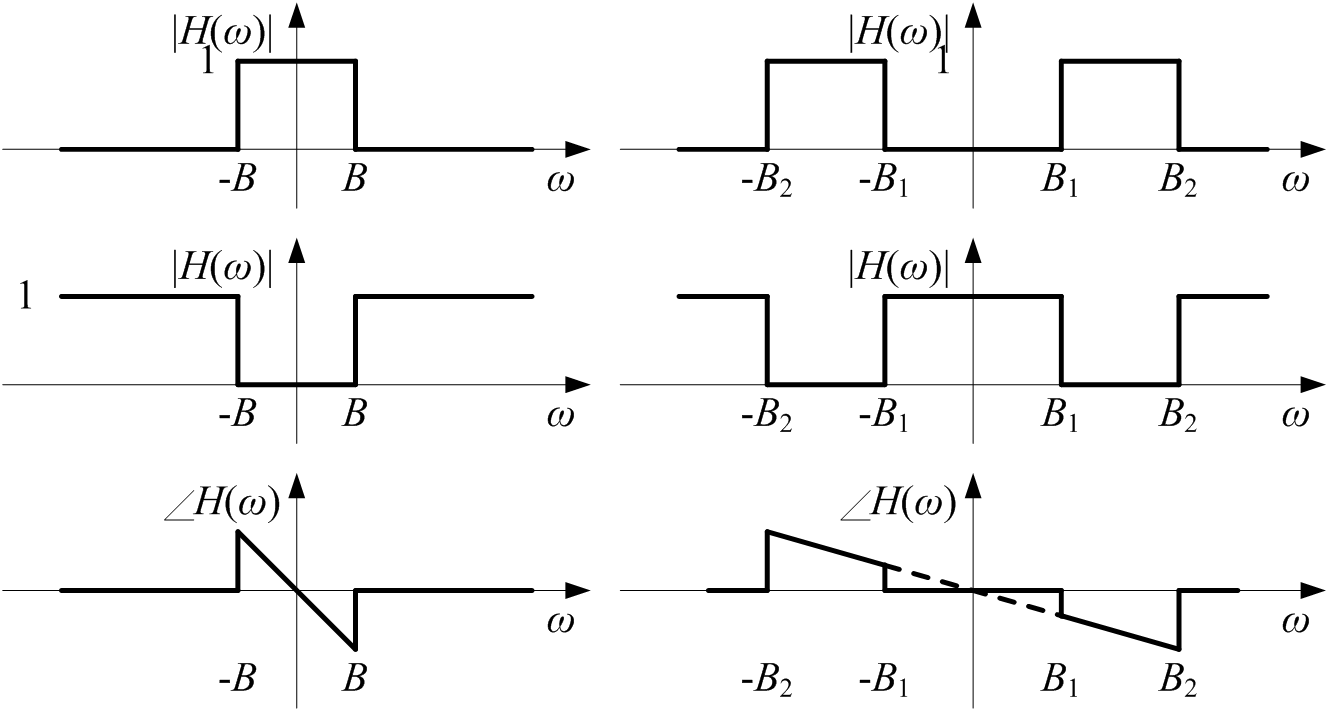
\includegraphics[height=6cm]{5.2.1-1.png}
\end{figure}

%============================================================
\subsection{理想低通滤波器的可能性}

理想的“全通”的频率响应应符合大小无衰减且相位线性,于是有:
\begin{align*}
&\because \begin{cases}
	\left| H\left( \omega \right) \right|=1\\
	\angle H\left( \omega \right) =-a\omega\\
\end{cases} \\
&\therefore H\left( \omega \right) =e^{ia\omega}
\end{align*}
则理想低通相当于全通被方波函数包络:
\[
H\left( \omega \right) =p_{2B}\left( \omega \right) \cdot e^{ia\omega}
\]
这是理想低通的频率响应。
根据傅里叶变换性质,系统的冲激响应:
\[
h\left( t \right) =\frac{B}{\pi}\mathrm{sinc}\frac{B\left( t-a \right)}{\pi}
\]
\begin{itemize}
    \item $B$:系统带宽;
    \item $a$:系统延时。
\end{itemize}
由于冲激响应在$t<0$都会有值,相当于作为输入的冲激还没有进系统,系统就有输出。
这种系统违反了因果律,所以理想低通是不存在的。






\newpage
\section{Nyquist采样定理}

本节简单介绍Nyquist采样定理。

假设信号$x\left( t \right) $,以$T$周期采样,采样后信号记为$x_s\left( t \right) $,则有:
\[
x_s\left( t \right) =\sum_{n=-\infty}^{+\infty}{x\left( t \right) \delta \left( t-nT \right)}
\]
假设信号的傅里叶变换$X\left( \omega \right) $,则采样信号$x_s\left( t \right) $的傅里叶变换有:
\[
X\left( \omega \right) =\sum_{n=-\infty}^{+\infty}{\frac{1}{T}X\left( t-n\omega _s \right)}
\]
其中,$\omega _s=2\pi /T$称为{\bf 采样频率}。
若信号在频域的带宽$B$有限,且采样频率满足$\omega _s>2B$,则采样本身不会对信号有任何影响,而且采样后的信号可以通过低通进行完全恢复,这就是{\bf Nyquist采样定理}。

Nyquist采样定理的前提是信号是有限带宽信号。
但实际信号因为时域有限而导致频域无限,本身就不满足Nyquist定理的先决条件,所以无论采样频率多高,都会使信号的高频发生混叠。
通常的做法是先让信号通过一个低通去掉高频,再进行采样。






\newpage
\section{Python应用}

本章的一个重点是能够借助Python,在频域角度分析系统对某输入的作用和输出结果。

本节要点:
\begin{itemize}
    \item 掌握Python分析方法。
\end{itemize}

%============================================================
\subsection{分析方法}

通常有一类问题是已知一个系统,要分析它的对信号产生的作用。
借助Python,一般步骤如下:
\begin{enumerate}
    \item 推导系统频域响应$H\left( \omega \right) $;
    \item 求解信号的傅里叶变换$X\left( \omega \right) $;
    \item 推导输出的时域函数$y\left( t \right) =\mathscr{F} ^{-1}\left[ H\left( \omega \right) \cdot X\left( \omega \right) \right] $。
\end{enumerate}

%============================================================
\subsection{例——RC电路分析}

\begin{example}
如下RC电路,设电压源为输入,电容两端电压为输出,分析不同的RC值对输出的影响。
\begin{figure}[h]
\centering
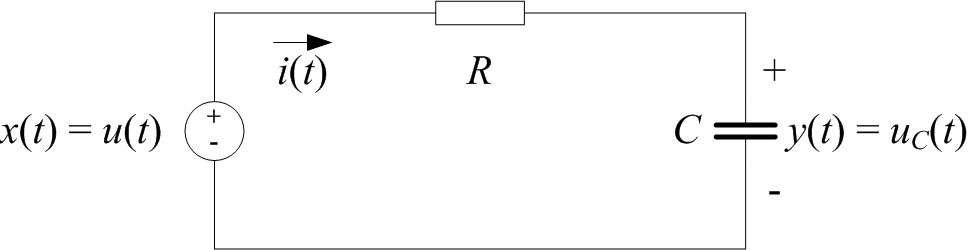
\includegraphics[height=2cm]{1.5.1-1.png}
\end{figure}
\[
x\left( t \right) =p_{\tau =1}\left( t \right) =\begin{cases}
	1,t\in \left[ -0.5,0.5 \right]\\
	0,t\notin \left[ -0.5,0.5 \right]\\
\end{cases}
\]
\end{example}

首先推导系统的频率响应,过程略:
\[
H\left( \omega \right) =\frac{1}{1+i\omega RC}
\]
分别取$RC=1,RC=0.1,RC=0.001$,系统频率响应的频谱图如下。
可见,减小电阻或电容都可以提高系统对高频的响应,特别在$RC=0.001$时,幅频图上看输出几乎没有衰减,相频图上看输出几乎没有相移。

\begin{python}
w  = np.arange(-50, 50, 0.01)
RC = 1;     H1 = 1 / (1 + RC * w * 1.0j)
RC = 0.1;   H2 = 1 / (1 + RC * w * 1.0j)
RC = 0.001; H3 = 1 / (1 + RC * w * 1.0j)

plot_mag_phs(w, np.abs(H1), np.angle(H1, deg=True),
             axs[0][0], axs[1][0], title=r"$H(\omega) ,RC=1$",     ...)
plot_mag_phs(w, np.abs(H2), np.angle(H2, deg=True),
             axs[0][1], axs[1][1], title=r"$H(\omega) ,RC=0.1$",   ...)
plot_mag_phs(w, np.abs(H3), np.angle(H3, deg=True),
             axs[0][2], axs[1][2], title=r"$H(\omega) ,RC=0.001$", ...)
\end{python}

\begin{figure}[h]
\centering
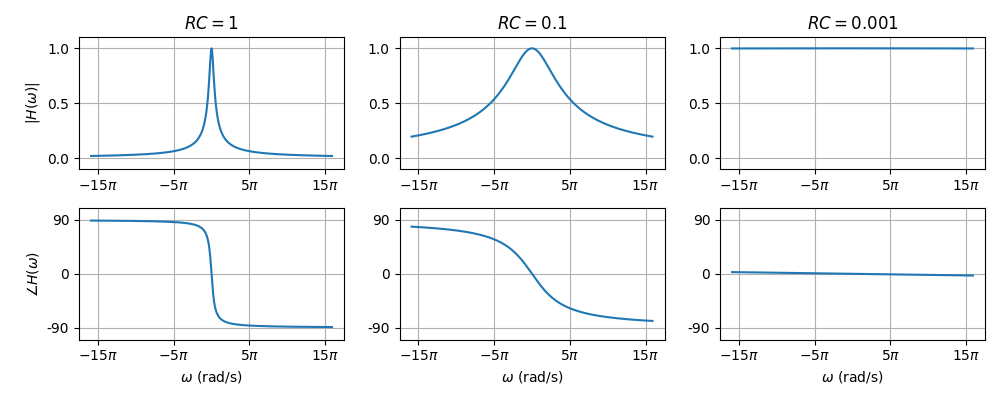
\includegraphics[height=4cm]{5.4.2-1.png}
\end{figure}

再分析输出信号的傅里叶变换,根据单方波的傅里叶变换计算输出的傅里叶:
\begin{align*}
&\because x\left( t \right) =p_{\tau =1}\left( t \right) \leftrightarrow X\left( \omega \right) =\frac{\sin \frac{\omega}{2}}{\frac{\omega}{2}} \\
&\therefore Y\left( \omega \right) =H\left( \omega \right) \cdot X\left( \omega \right) =\frac{1}{1+i\omega RC}\cdot \frac{\sin \frac{\omega}{2}}{\frac{\omega}{2}}
\end{align*}
取$RC=0.5,RC=0.001$,输入和输出的频谱图如下,$RC:0.5\rightarrow 0.001$提高了对输入信号高频部分的响应,使得输出更像输入。
\begin{figure}[h]
\centering
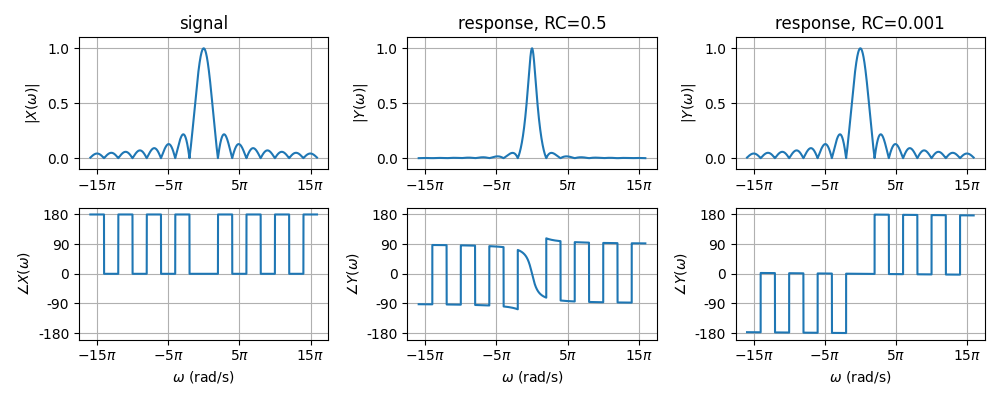
\includegraphics[height=4cm]{5.4.2-2.png}
\end{figure}

\begin{python}
w  = np.arange(-50, 50, 0.01)
X  = (np.sin(w/2) / (w/2))
RC = 0.5;   Y1 = 1 / (1 + RC * w * 1.0j) * (np.sin(w/2) / (w/2))
RC = 0.001; Y2 = 1 / (1 + RC * w * 1.0j) * (np.sin(w/2) / (w/2))

plot_mag_phs(w, np.abs(X),  np.angle(X, deg=True),
             axs[0][0], axs[1][0], title=r"$X(\omega)$",           ...)
plot_mag_phs(w, np.abs(Y1), np.angle(Y1, deg=True),
             axs[0][1], axs[1][1], title=r"$Y(\omega) ,RC=0.5$",   ...)
plot_mag_phs(w, np.abs(Y2), np.angle(Y2, deg=True),
             axs[0][2], axs[1][2], title=r"$Y(\omega) ,RC=0.001$", ...)
\end{python}









